% Copyright(C) 2013, Andreas Halle
\documentclass[preview]{standalone}
\usepackage{pgf}
\usepackage{tikz}
\usetikzlibrary{automata}
\begin{document}
\pagestyle{empty}

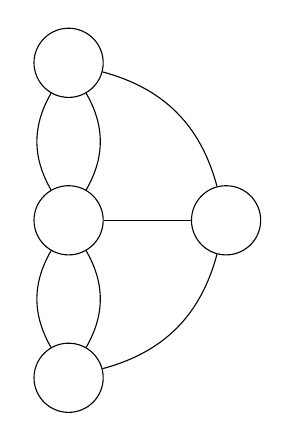
\begin{tikzpicture}[node distance=2cm]
    \tikzstyle{every state}=[draw]

    \node[state] (a) {};
    \node[state] (b) [below of=a] {};
    \node[state] (c) [below of=b] {};
    \node[state] (d) [right of=b] {};

    \path (a) edge [bend left]  node {} (b)
          (a) edge [bend right] node {} (b)
          (a) edge [bend left]  node {} (d)
          (b) edge [bend left]  node {} (c)
          (b) edge [bend right] node {} (c)
          (b) edge              node {} (d)
          (c) edge [bend right] node {} (d);
\end{tikzpicture}
\end{document}
